Este capítulo apresenta o problema identificado, a proposta de resolução para este problema, o planejamento de ações para alcançar a solução e os resultados que são esperados ao fim da pesquisa.



\section{Metodologia}
\label{sec:methodology}

 Para a resolução do problema apresentado, é proposto a criação de uma ontologia que contemple  as propriedades necessárias de pacientes a serem atendidos em uma especialidade médica e um protótipo que utilize estes itens e gerencie uma fila de espera de acordo com critérios preestabelecidos por médicos.

    Com o intuito de validar a proposta, será desenvolvido um estudo de caso com o Hospital das Clínicas da Faculdade de Medicina de Marília (FAMEMA), onde se espera implantar a ontologia e o protótipo. Posteriormente solicitar a médicos que avaliem o gerenciamento realizado pelo protótipo, e informem qual a concordância com a fila gerenciada de acordo com a quantidade de pacientes que julgarem estar corretamente posicionados, e para efeito de comparação também informarem qual a concordância da fila de atendimento gerenciada antes da implantação do protótipo, permitindo assim analisar se a proposta de fato pode gerenciar uma fila de espera de forma mais eficaz na visão dos especialistas (médicos).
	
	O intuito não é discutir quais deverão ser critérios utilizados pelos médicos para avaliar se um paciente X tem prioridade em relação ao paciente Y, mas sim possibilitar que a partir de critérios previamente estabelecidos, o computador possa fazer esta triagem de forma eficaz, sem a necessidade de alocação de um médico para uma avaliação caso a caso, e nem que funcionários administrativos façam esse ordenamento, almejando um ordenamento mais próximo ao que os médicos aconselham, sendo mais justa e transparente uma fila de atendimento. 
	
	O método para se chegar ao objetivo desta pesquisa é utilizar recursos da web semântica, como a ontologia para que se possa representar itens de pacientes que poderão ser utilizados para gerenciar uma fila de espera.

    \section{Cronograma}

	Considerando um tempo de 25 meses para o desenvolvimento da pesquisa proposta e a numeração das tarefas apresentadas na \autoref{sec:methodology}, o cronograma das atividades se apresenta na Tabela 1 %\autoref{tab:cronogram}.
	
	  \begin{enumerate}
    	\item Conclusão da validação do exame de proficiência em língua estrangeira;
        \item Integralização dos créditos obrigatórios;
        \item Mapeamento da literatura;
        \item Elaboração e apresentação dos artefatos relacionados ao exame de qualificação;
         \item Desenvolvimento da ontologia OWL que represente indicadores para classificação de prioridades para o atendimento de uma especialidade médica;
        \item Desenvolvimento e testes de um protótipo que utilize a ontologia desenvolvida e gerencie uma fila de espera utilizando critérios definidos;
        \item Elaboração e submissão de artigos;
        \item Elaboração e apresentação dos artefatos relacionados a defesa;
    \end{enumerate}
    
    \begin{table}[htbp]
    	\centering
        \caption{Cronograma das atividades da pesquisa.}
        \label{tab:cronogram}
        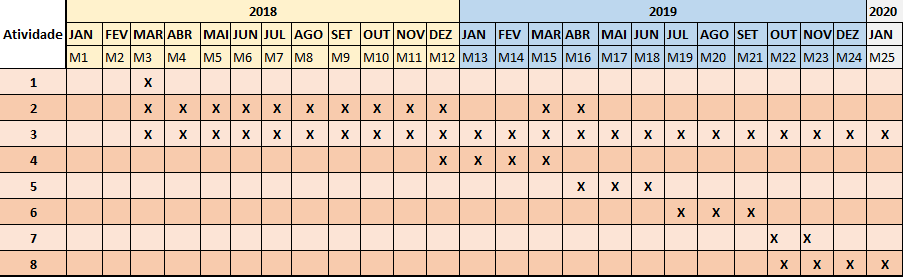
\includegraphics[width=1\linewidth]{images/cronogram}
        \fautor
    \end{table}
    
    \pagebreak
    
   \section{ Resultados Esperados}

	Ao final desta pesquisa espera-se as seguintes contribuições:
	
	\begin{itemize}
		\item Uma ontologia OWL que represente indicadores para classificação de prioridades para o atendimento de uma especialidade médica;
        \item  Um protótipo que gerencie filas de espera computacionalmente e se mostre  mais eficaz que o gerenciamento atual do HC FAMEMA;
        \item Estudo de caso mostre que o modelo proposto pode auxiliar na gestão de filas do Sistema Único de Saúde e obter benefícios se comparadas as outras formas de gerenciamento;
	\end{itemize}
